\documentclass{bioinfo}
\usepackage{natbib}
\copyrightyear{2009}
\pubyear{2009}

\newcommand{\Rpackage}[1]{`\texttt{#1}'}
\newcommand{\Rclass}[1]{\textsl{#1}}
\newcommand{\subfig}[1]{\textbf{#1}}

\begin{document}
\firstpage{1}

\title[Modular analysis]{Modular analysis of gene expression data with
  GNU R}
\author[G\'abor Cs\'ardi \textit{et~al}]{G\'abor Cs\'ardi\,,$^{1,2}$,
  Zolt\'an Kutalik\,$^{1,2}$ and Sven Bergmann\,$^{1,2}$}
\address{$^{1}$Department of Medical Genetics, and 
  $^{2}$Swiss Institute of Bioinformatics,
  University of Lausanne, Rue de Bugnon 27, CH-1005 Lausanne,
  Switzerland.}

\history{Received on XXXXX; revised on XXXXX; accepted on XXXXX}

\editor{Associate Editor: XXXXXXX}

\maketitle

\begin{abstract}
TODO
\section{Summary:} TODO
\section{Availability:}
\href{http://www.unil.ch/cbg/homepage/software.html}%
{http://www.unil.ch/cbg/homepage/software.html}
\section{Contact:} \href{Sven.Bergmann@unil.ch}{Sven.Bergmann@unil.ch}
\end{abstract}

\section{Introduction}

% What is biclustering.

Biclustering is the idea of clustering the rows and the columns of a
data matrix together, usually not independently. In other words, the
goal of a biclustering algorithm is to find blocks in the reordered
data matrix that have, such that the blocks have correlated rows and
columns. It is important to note that these blocks (or biclusters,
modules) have context, i.e. the rows only need to be correlated across
the columns of the block, but not across other columns of the data
matrix; and vice-versa.

When it comes to gene expression data, a bicluster means a subset of
genes ($G$) (or probes, probe sets) and a subset of samples ($S$),
such that genes $G$ are exactly coexpressed across $S$ and samples $S$
have correlated expression profile exactly across $G$.

% What is the ISA.

The Iterative Signature Algorithm (ISA), \cite{sa,isa,isamod}, is a 
powerful biclustering algorithm. It is able to identify biclusters
that overlap and it is resilient to noise.

In this short note, we introduce the \Rpackage{isa2} and
\Rpackage{eisa} GNU R, \cite{R}, packages; these implement the ISA
biclustering method, provide a convenient interface to run it using
the BioConductor, \cite{BioC}, software package, and also contain
visualization tools.

\section{Methods}

\begin{figure*}
\centering
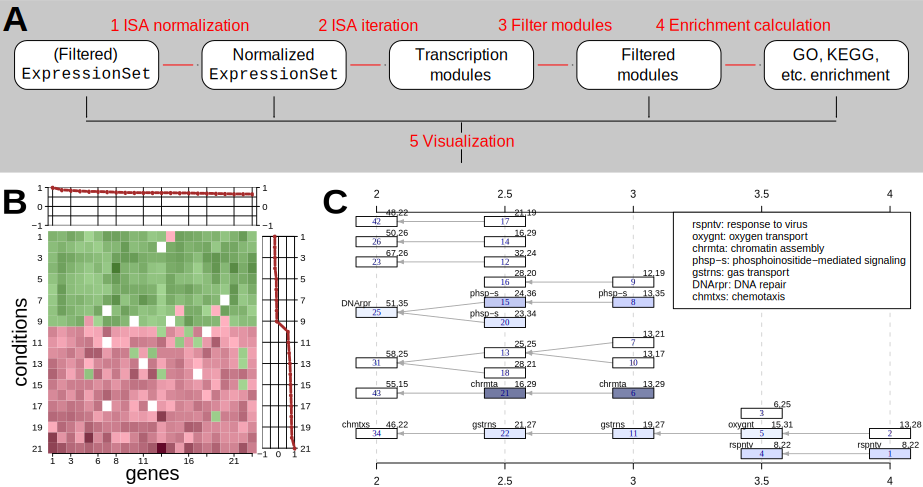
\includegraphics[width=0.9\textwidth]{isa2workflow3}
\caption{Work flow of a typical modular analysis study, with the
  \Rpackage{eisa} package (left); and four bicluster visualization
  techniques (right). The input of the \Rpackage{eisa} pipeline is a
  BioConductor \Rclass{ExpressionSet} object. This is normalized to
  $Z$-scores (1); the ISA iteration is performed on it using smart or
  random seeds (2); and the biclusters are then merged and filtered
  based on the robustness measure (3). The \Rpackage{eisa} package
  contains tools to perform many GO, KEGG, etc. enrichment calculation
  quickly (4), and several bicluster visualization tools (5).
  Subfigures \subfig{A}, \subfig{B}, \subfig{C} and \subfig{D} were generated
  using the acute lymphoblastic leukemia data set, see
  \cite{chiaretti04} and the \Rpackage{ALL} R package.
  \subfig{(A)} A condition plot for a simple bicluster. Each sample is
  represented as a bar, its height is its score in the bicluster. 
  Samples above the red (none in this case) and samples
  below the green line are part of the biclusters. The coloring
  indicates cases and controls. This module can separate control and
  case samples.
  \subfig{(B)} A module tree. Each rectangle is a bicluster. See the
  definition of the module tree in the text. The modules are colored
  according to their Gene Ontology enrichment $p$-values, the codes of
  the enriched GO categories are shown in the top-left corner of the
  rectangles. The top-right corner shows the number of genes and
  conditions in the bicluster. The numbers on the horizontal axes are
  the gene thresholds used for finding the modules.
  \subfig{(C)} Heatmap for a single module, showing correlated
  expression and the genes and samples. The red lines are the gene and
  sample scores.
  \subfig{(D)} Profile plot, for a single module. On the top plot the
  expression of all samples are plotted, the samples of the module
  with black. The red and green lines show the mean of the two
  groups. The bottom plot is the same for the genes of the module.
}
\label{fig:workflow}
\end{figure*}

Let us first explain the briefly the steps of a typical modular
analysis study for gene expression data.

% Batch correction
\paragraph{Batch correction}
Often, the ISA is applied to samples from different experiments. In
this case it is crucial to address the question of experimental
variation. Several methods exist to solve this problem,
see e.g. \cite{johnson07} for an algorithm that has a GNU R
implementation.

% Filtering
\paragraph{Gene filtering}
Depending on the application, it can be advantageous to remove genes
that are not expressed in any of the samples, especially because the
ISA normalization (next step) tends to amplify their effect.

% Normalization. 
\paragraph{ISA normalization}
ISA is an iterative algorithm. In each step it computes weighted sums
of expression levels for a number of genes or a number of
samples. Since different genes typically show different levels of base
expression and variance, it is important to standardize expression
levels to $Z$-scores. The ISA uses two sets of $Z$-scores, one
calculated for each gene across all samples, the other for each sample
across all genes.

% Random and smart seeding.
\paragraph{Random and smart seeding}
The ISA used with random seeds is an unsupervised algorithm, it uses no
external knowledge to find the biclusters. ISA with smart seeds is
biased towards genes or pathways of interest, or sample annotation.
This latter form can be considered as a semi-supervised approach.

% The ISA iteration. 
\paragraph{The ISA iteration}
This step is essentially performing the ISA and finding the biclusters
from the starting seeds.

% Merging the modules.
\paragraph{Merging the modules}
It is possible that more seeds converge to the same, or very similar
biclusters. This step eliminates such duplicates.

% The robustness measure and filtering the modules. 
\paragraph{Robustness of biclusters}
To access the significance of a bicluster, we designed a robustness
measure, that can be used to filter out spurious modules. This is done
based on performing ISA on the scrambled input data.

% Module trees.
\paragraph{Module trees}
The ISA works with two stringency threshold parameters, the gene
threshold and the sample threshold. ISA modules can be organized into
a directed graph, a module tree, in which there is an edge from module
$A$ to module $B$, if the ISA converges to module $B$ from module $A$,
with the same threshold parameters  that were used to find module
$B$. A module tree provides a hierarchical modular description of a
data set.

\section{Implementation}

The ISA and accompanying visualization tools are implemented in two R
packages. The \Rpackage{isa2} package contains the implementation of
the basic ISA itself; this package can be used to analyze any tabular
data. The \Rpackage{eisa} package builds on \Rpackage{isa2}. It adds
support to standard BioConductor gene expression data structures; and
contains gene expression specific visualization tools, see some of
these in Fig.~\ref{fig:workflow}.

Both the \Rpackage{isa2} and \Rpackage{eisa} packages support two
workflows. The \emph{simple workflow} involves a single R function
call and runs all ISA steps (1-3 on Fig.~\ref{fig:workflow}.) with
their default parameters.

The \emph{detailed workflow} means running every step of the modular
analysis separately, possibly with non-default parameters. This allows
the users to tailor the ISA completely according their needs.

For users that prefer Matlab over R, we created a Matlab package for
ISA, please see the ISA homepage for more information.

% \subsubsection{Visualization}

The \Rpackage{eisa} package implements a set of visualization
techniques for biclusters, some of these are specific to ISA, others
are not. Please see Fig.~\ref{fig:workflow} for some of these.

The \Rpackage{ExpressionView} R package implements an interactive tool
for visualizing ISA (or other) overlapping biclusters.

% \subsubsection{Connection to other software}

The \Rpackage{biclust} package, \cite{biclust}, implements a number of
biclustering algorithms in a unified framework. The \Rpackage{eisa}
package include tools to convert between \Rpackage{biclust} and ISA
biclusters. This allows the cross-talk of the functions in the two
packages.

\section*{Acknowledgement}

TODO

\paragraph{Funding\textcolon} TODO

\paragraph{Conflict of interest\textcolon} None declared.

\bibliographystyle{natbib}
\bibliography{isa}

\end{document}
